%\chapter*{Неделя 5}
\protect\thispagestyle{fancy}
\section{}
Для узкополосного случайного процесса со спектром шириной $\Delta \omega$ сосредоточенным возле частот $\pm \omega_0$ определить и изобразить корреляционную функцию $\Capit{R}(\tau)$.

\begin{figure}[!h]
	\centering
	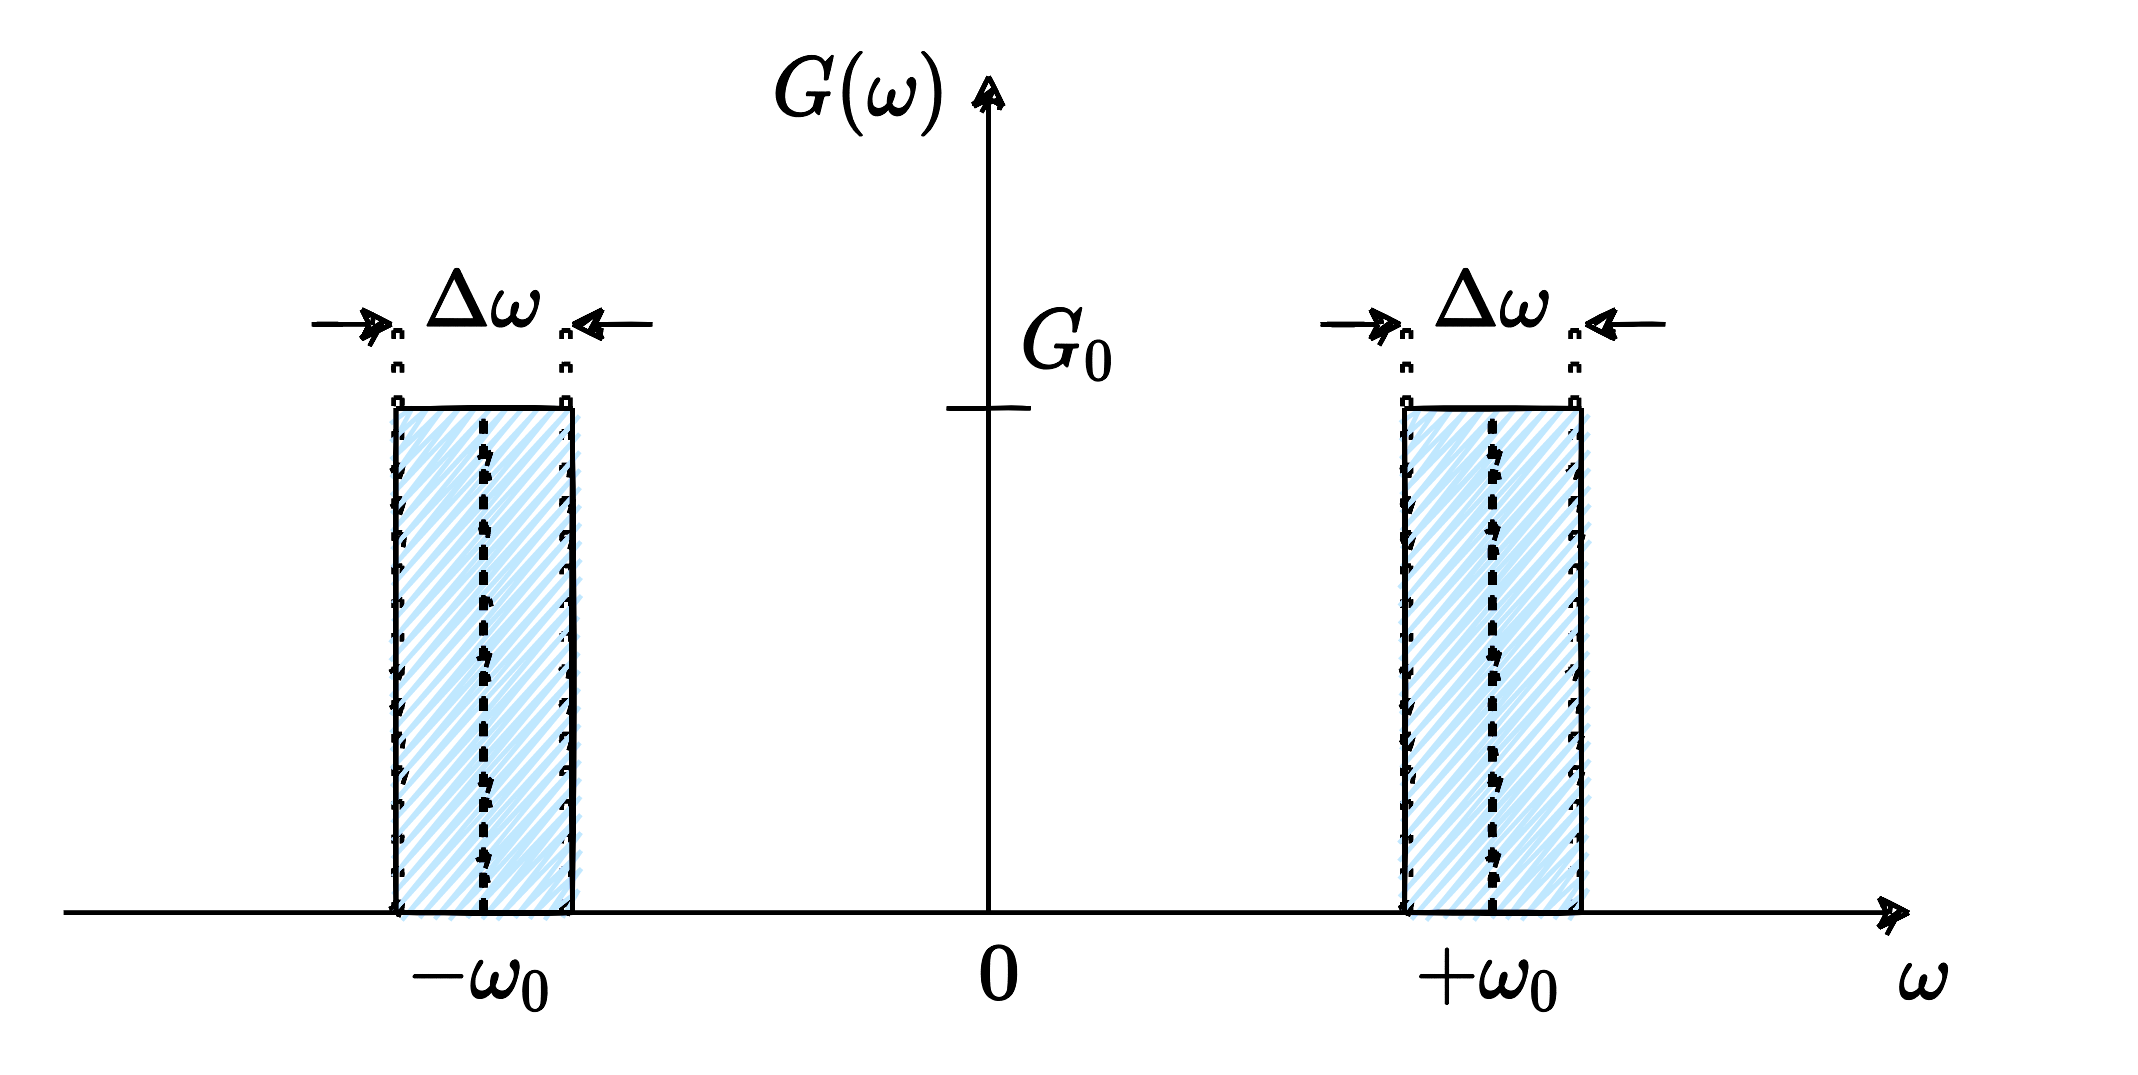
\includegraphics[width=0.65\columnwidth]{pics/spring/5/1-0.png}
	%\caption{.}
	\label{fig:5-1-0}
\end{figure}


\begin{align*}
\Capit{R}(\tau) &= \dfrac{1}{2\pi}\int \limits_{-\infty}^{+\infty} G(\omega)e^{j\omega \tau}d\omega =
\dfrac{1}{\pi}\int \limits_{0}^{+\infty} G(\omega)\cos(\omega \tau)d\omega =
\dfrac{1}{\pi}\int \limits_{\omega_0 - \Delta \omega/2}^{\omega_0 + \Delta \omega/2} G_0\cos(\omega \tau)d\omega =
\dfrac{G_0}{\pi\tau}\int \limits_{\omega_0 - \Delta \omega/2}^{\omega_0 + \Delta \omega/2}d\sin(\omega \tau) = \\ &=
\dfrac{G_0}{\pi\tau} \sin(\omega \tau) \Bigg|_{\omega_0 - \Delta \omega/2}^{\omega_0 + \Delta \omega/2}=
\dfrac{G_0}{\pi\tau} \big[ \sin((\omega_0 + \Delta \omega/2)\tau) - \sin((\omega_0 - \Delta \omega/2)\tau)\big] = 
\dfrac{2G_0}{\pi\tau} \cos (\omega_0 \tau) \sin\left(\dfrac{\Delta \omega \tau}{2}\right) =\\&=
\dfrac{\Delta \omega G_0}{\pi} \cos (\omega_0 \tau) \cdot \dfrac{\sin\left(\dfrac{\Delta \omega \tau}{2}\right)}{\dfrac{\Delta \omega\tau}{2}} =
\dfrac{\Delta \omega G_0}{\pi} \cos (\omega_0 \tau)\cdot \sinc\left(\dfrac{\Delta \omega \tau}{2}\right).
\end{align*}



\begin{figure}[!h]
	\centering
	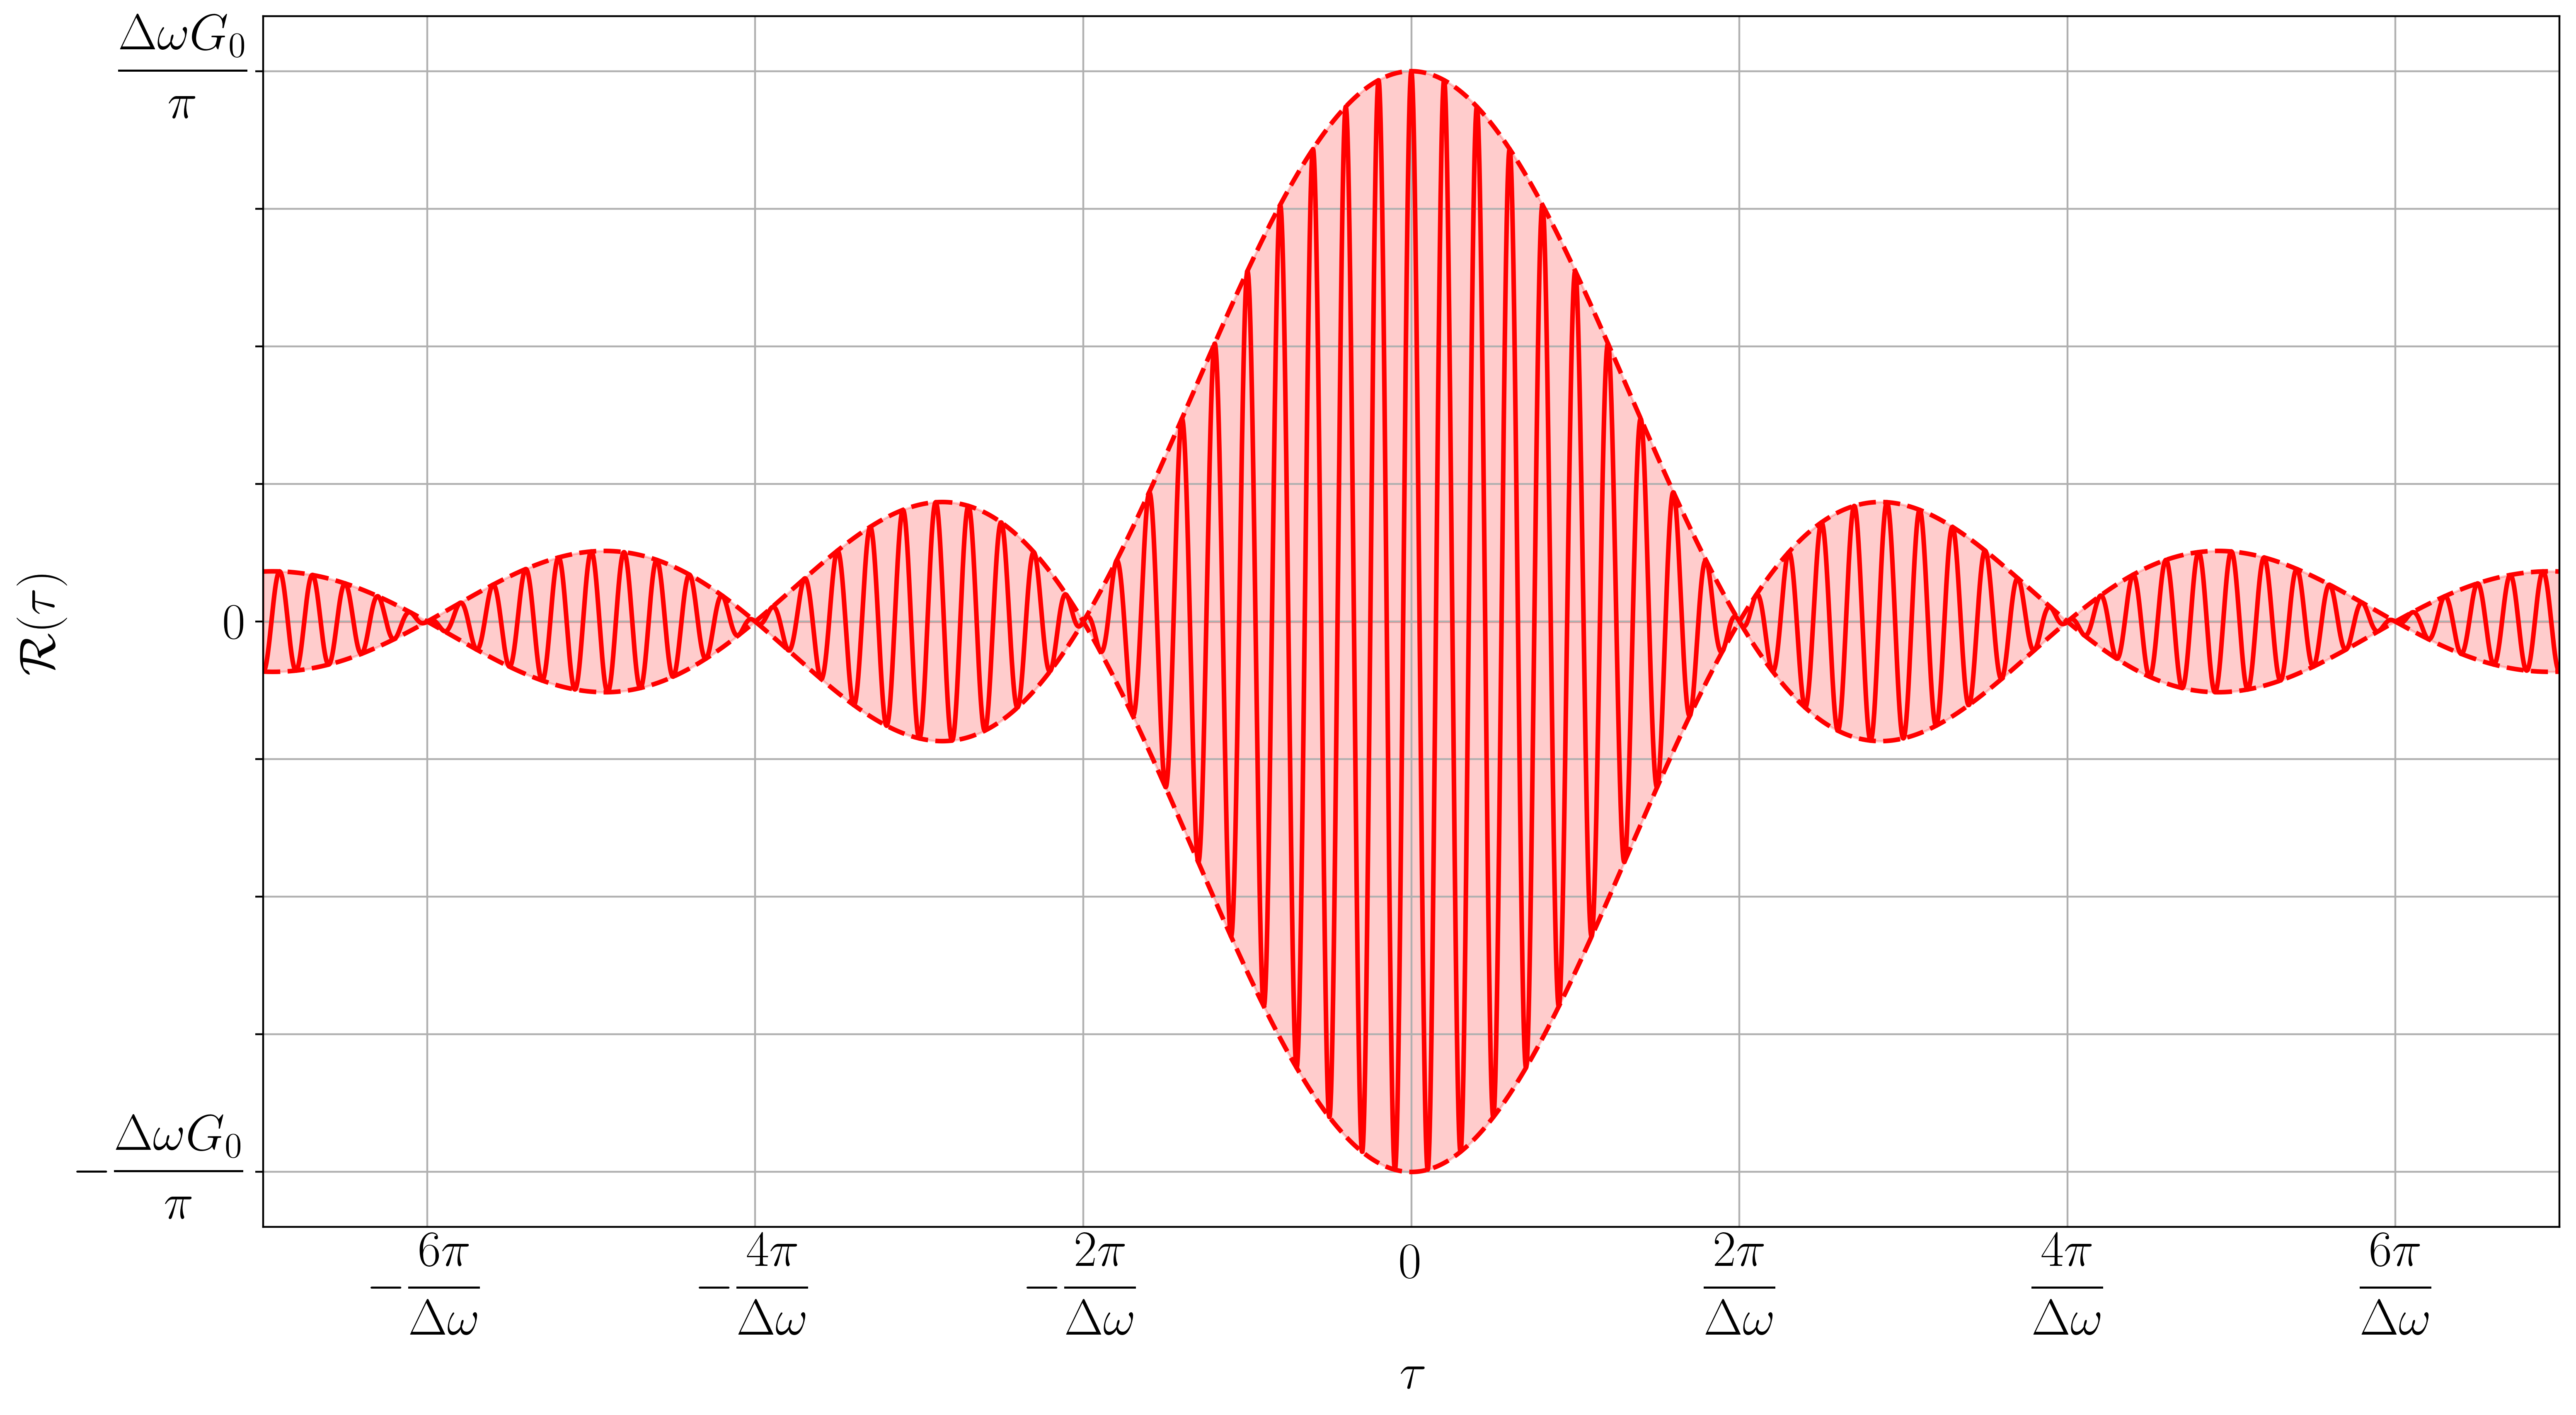
\includegraphics[width=0.9\columnwidth]{pics/spring/5/1.png}
	%\caption{.}
	\label{fig:5-1}
\end{figure}

\newpage
\section{}
Случайный процесс имеет экспоненциальную функцию корреляции
\begin{equation*}
\Capit{R}(\tau) = \sigma^2 e^{-\alpha |\tau|},\quad \alpha>0.
\end{equation*}

Определить и изобразить спектральную плотность мощности $G(\omega)$.

\begin{align*}
G(\omega) &= \int \limits_{-\infty}^{+\infty}\Capit{R}(\tau)e^{-j\omega\tau}d\tau =
\int \limits_{-\infty}^{+\infty}\sigma^2 e^{-\alpha |\tau|}e^{-j\omega\tau}d\tau =
\int \limits_{-\infty}^{0}\sigma^2 e^{+\alpha \tau}e^{-j\omega\tau}d\tau + 
\int \limits_{0}^{+\infty}\sigma^2 e^{-\alpha \tau}e^{-j\omega\tau}d\tau =\\&=
\int \limits_{-\infty}^{0}\sigma^2e^{(\alpha - j\omega) \tau}d\tau + 
\int \limits_{0}^{+\infty}\sigma^2e^{-(\alpha + j\omega)\tau}d\tau =
\sigma^2 \dfrac{e^{(\alpha - j\omega)t}}{(\alpha - j\omega)}\Bigg|_{-\infty}^{0} -
\sigma^2 \dfrac{e^{-(\alpha + j\omega)t}}{(\alpha + j\omega)}\Bigg|_{0}^{+\infty} = \\&=
\sigma^2 \left\{ \dfrac{1}{(\alpha - j\omega)} + \dfrac{1}{(\alpha + j\omega)}\right\} =
\dfrac{2 \alpha \sigma^2}{\alpha^2 + \omega^2}.
\end{align*}


\begin{figure}[!h]
	\centering
	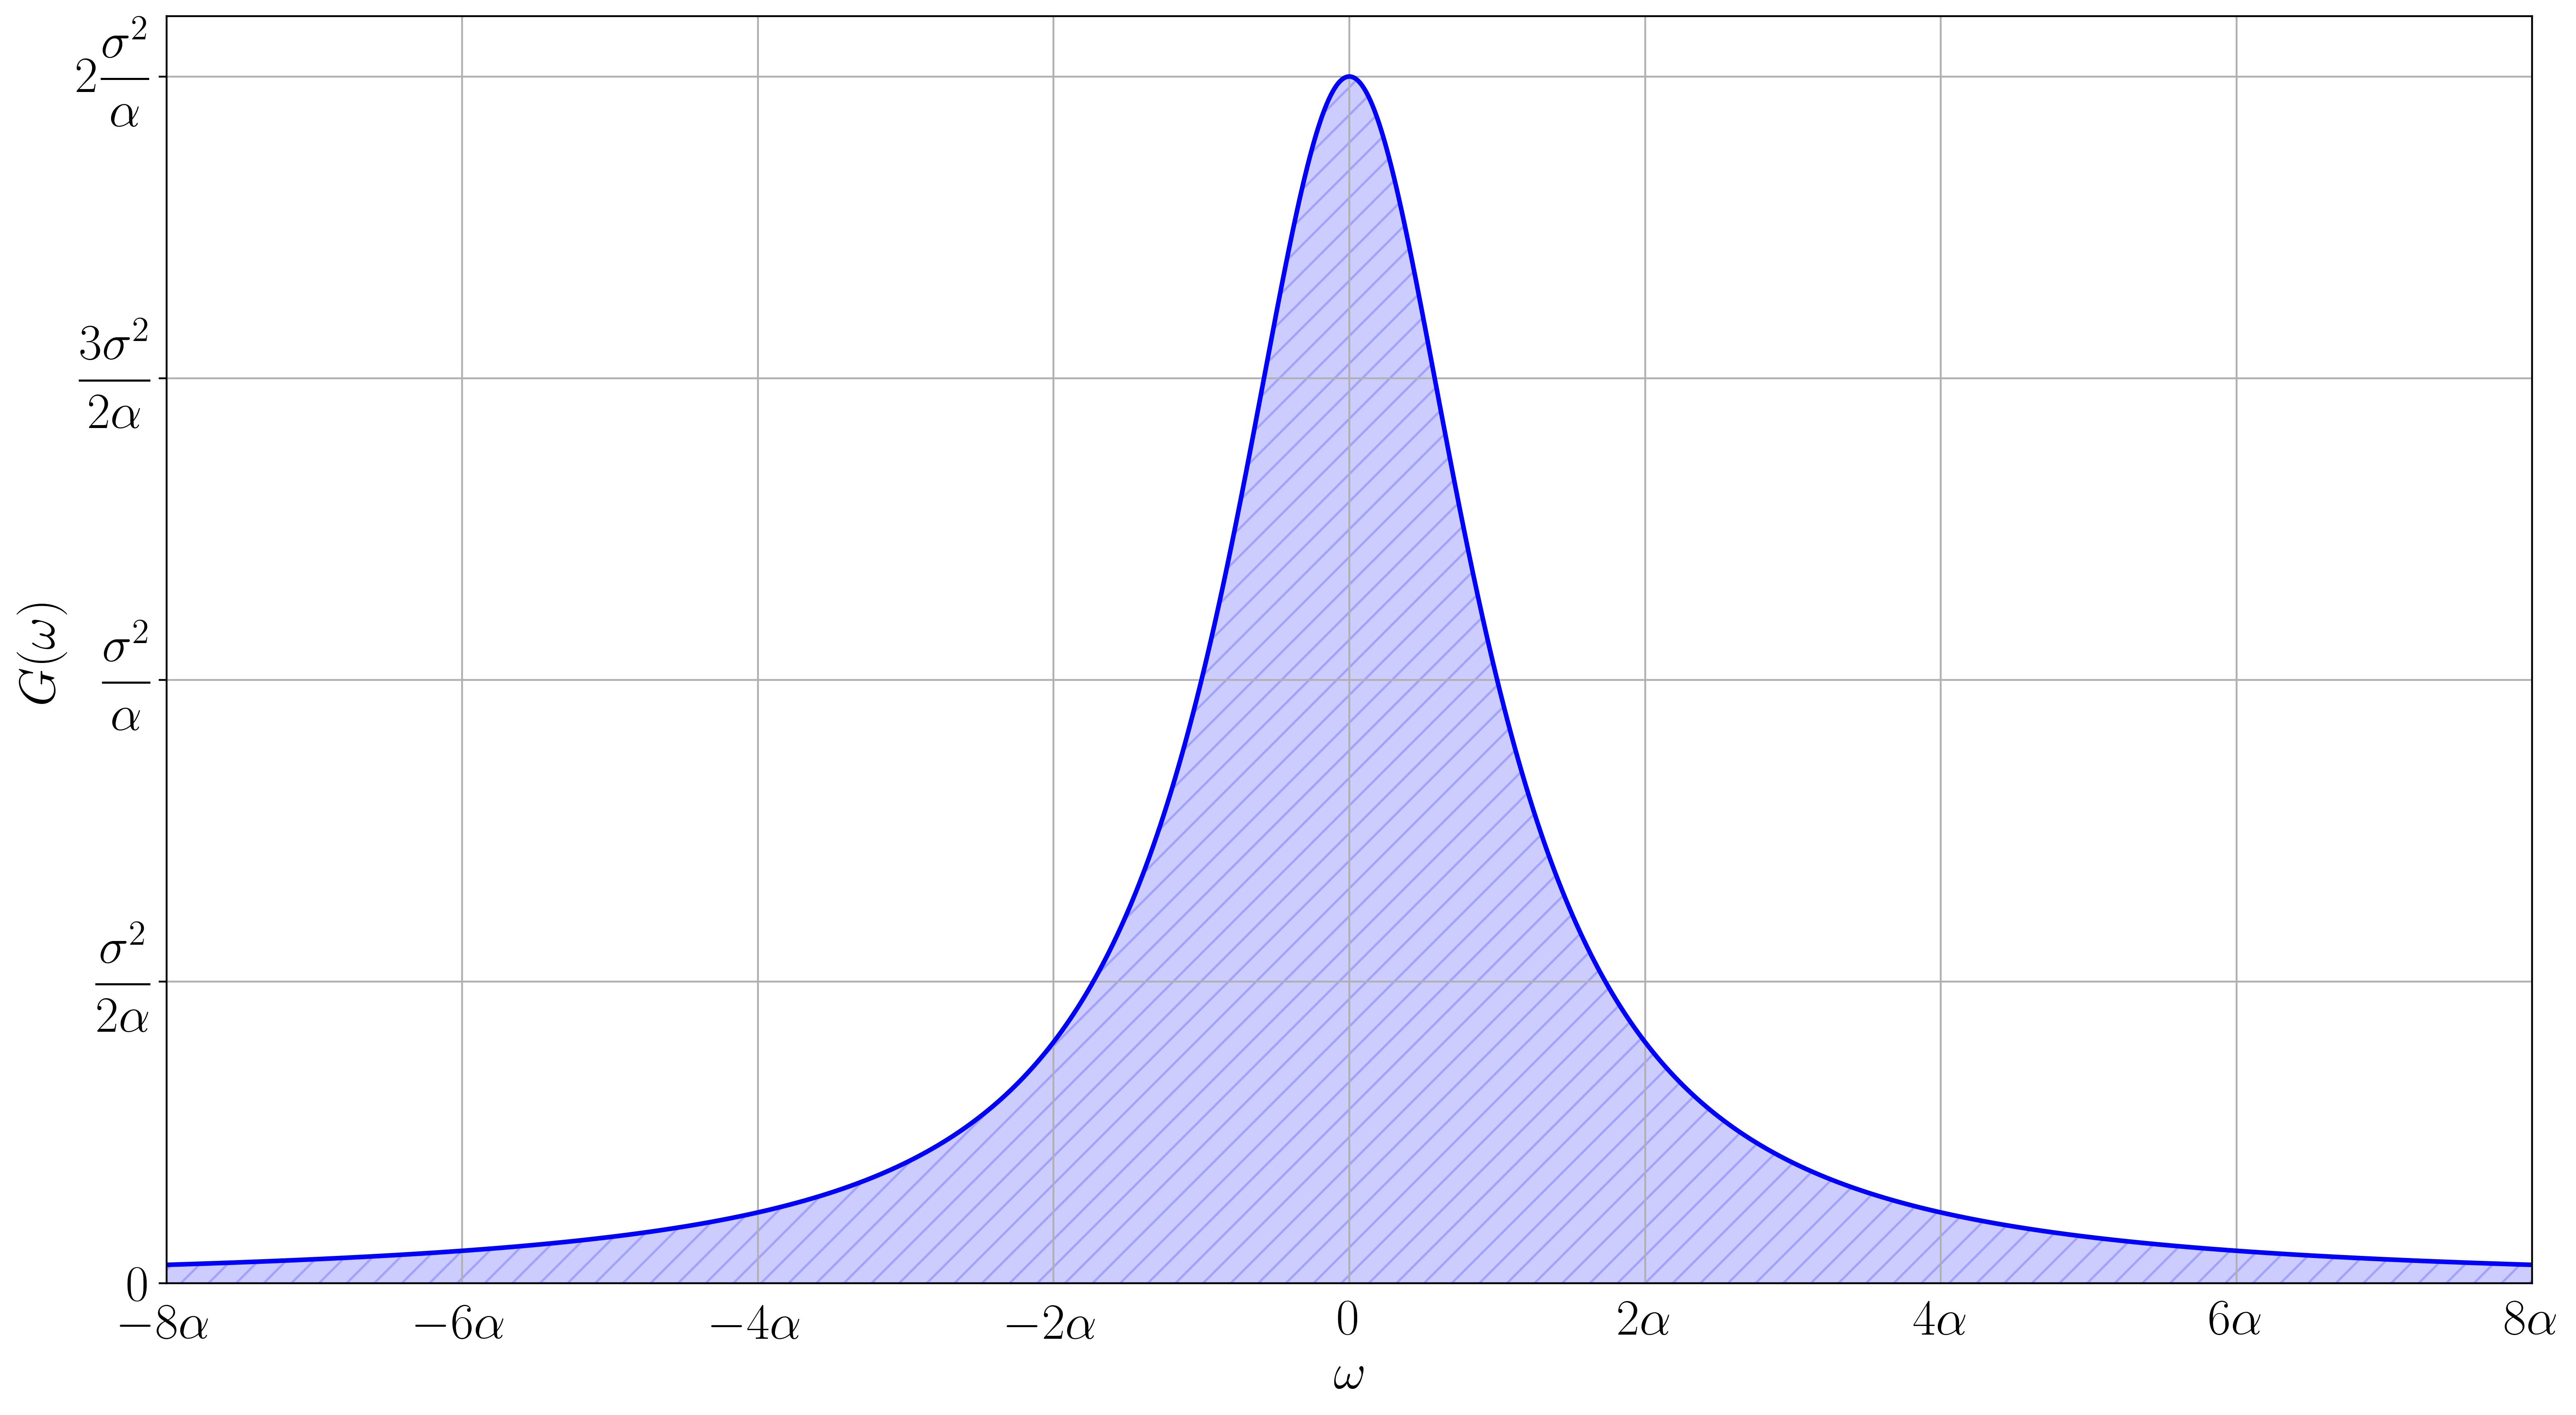
\includegraphics[width=0.9\columnwidth]{pics/spring/5/2.png}
	%\caption{.}
	\label{fig:5-2}
\end{figure}

\newpage
\section{}

\begin{itemize}
	\item Дайте определение СПМ.
	
	Спектральная плотность мощности (СПМ) для некоторой реализации сигнала $x(t)$ задаётся следующим соотношением:
	\begin{equation*}
	G(\omega) = \lim_{T \to +\infty} \dfrac{1}{T}\mathbb{E}\left\{\Bigg|\int \limits_{-T/2}^{+T/2}x(t)e^{-j\omega t}dt\Bigg|^2 \right\}.
	\end{equation*}
	По своему определению $G(\omega)$ есть вещественная неотрицательная функция частоты.
	Функция спектральной плотности мощности задаёт среднюю мощность, сосредоточенную в полосе частот шириной $1$ Hz на центральной циклической частоте $\omega$. 
	
	
	\item Почему на практике доступны для анализа только оценки СПМ?
	
	Поскольку в реальности бесконечное время моделирования недостижимо, а число доступных случайных реализаций ограничено, на практике приходится работать лишь с оценками спектральной плотности мощности какого-либо сигнала.
\end{itemize}
